In recent years rehabilitation medicine, and prosthetics in
particular, has benefited from the advances in mechatronics, a field
which exquisitely pertains to robotics and mathematics. This synergy
is driving rehabilitation medicine to a scenario in which an amputee's
life will be better, when more dexterous and controllable prostheses
will make it to the market. The paradigmatic example is represented by
the recent commercialisation of Touch Bionics's i-LIMB prosthetic hand
\cite{ilimb}, which is lightweight, long-running, it has five fingers
and five degrees of freedom (one per finger, see Figure
\ref{fig:hands} $(a)$). (At the time of writing, a few hundreds i-LIMBs
have been implanted and sold.)

\begin{figure}
  \begin{tabular}{ccc}
    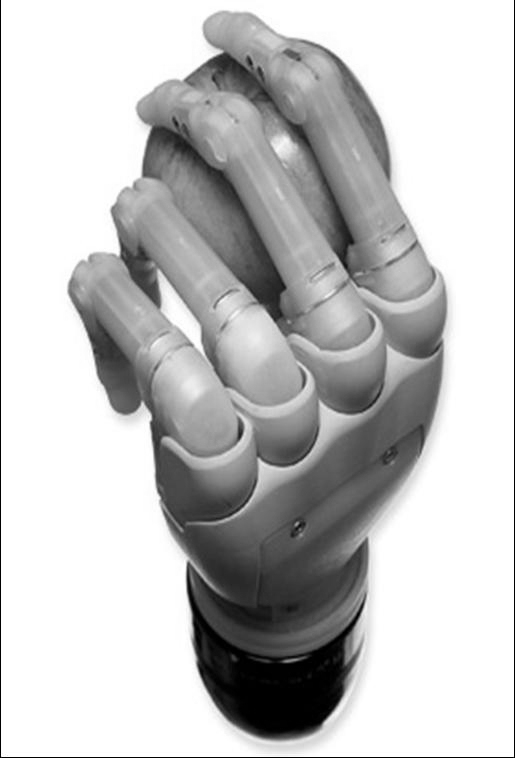
\includegraphics[width=0.14\textwidth]{figs/hands_TB.jpg} &
    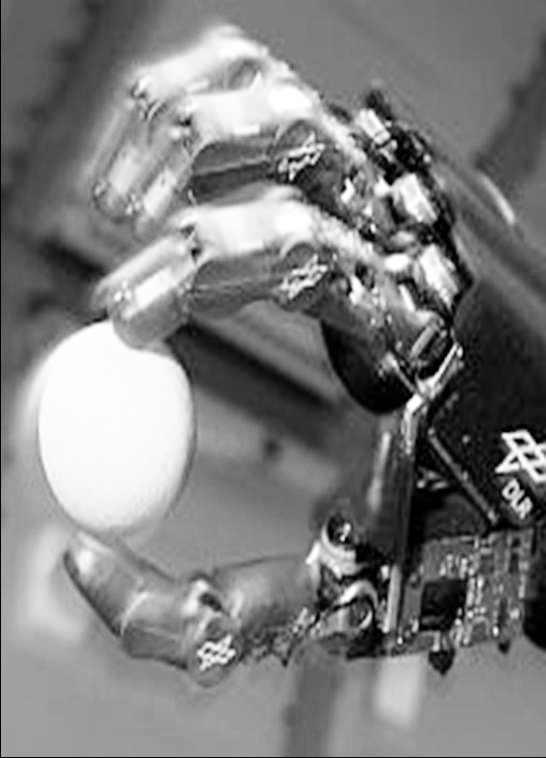
\includegraphics[width=0.14\textwidth]{figs/hands_DLRII.jpg} &
    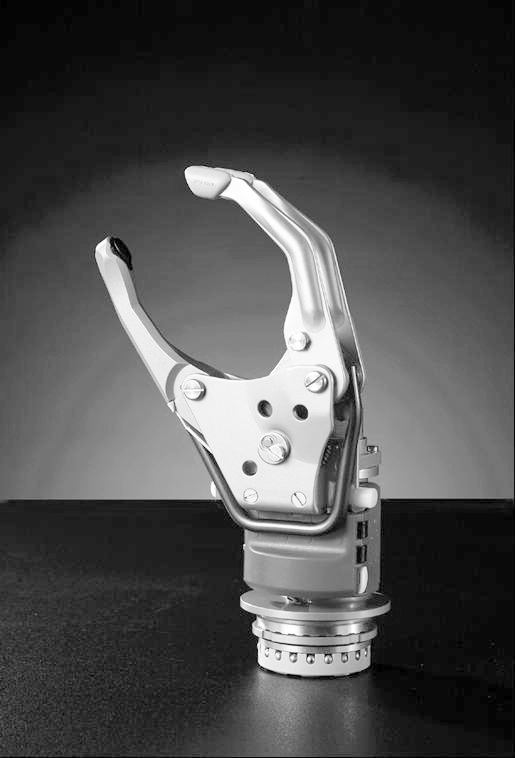
\includegraphics[width=0.14\textwidth]{figs/hands_OB.jpg} \\
    $(a)$ & $(b)$ & $(c)$
  \end{tabular}
  \caption{$(a)$ Touch Bionics's i-LIMB prosthetic hand (reproduced
    from \cite{ilimb}; $(b)$ the DLR-II mechanical hand; $(c)$ Otto
    Bock's SensorHand Speed (reproduced from \cite{sensorhand}).}
  \label{fig:hands}
\end{figure}

The dexterity of this prosthesis is very high, though still far from
the best non-prosthetic robot hand prototypes (e.g., the DLR-II hand,
see \cite{Hua2006} and Figure \ref{fig:hands} $(b)$). In fact, it
represents a real breakthrough with respect to the state-of-the-art
commercial prostheses, namely Otto Bock's SensorHand Speed (see Figure
\ref{fig:hands} $(c)$), which has one open/close DOF.

Still, \emph{control} is far from optimal. The most widely used control
device nowadays is surface electromyography (EMG), a cheap,
non-invasive technique by which surface electrodes gather from the
patient's stump skin the (residual) muscle activation potentials (see,
e.g., \cite{deluca}); these potentials are then somehow translated to
motor commands. The current control strategies employ large muscles,
such as the wrist flexor/extensor, to control one or, at best, two
DOFs (e.g., opening and closing of the Otto Bock's claw). This implies
long training times for the patient, and results in poor control.

Even a dexterous hand prosthesis as the i-LIMB cannot be controlled in
a fine and natural way; it uses two EMG electrodes in combination, to
produce a set of predefined grasp shapes; and the force involved in
the grasp is not controlled. Most of the adaptability is left to the
compliance of the hand itself. Notice that \emph{force control} is a
paramount requirement in Daily-Life Activities (DLA): picture the
possibility of holding an egg without breaking it, of hoding a hammer
without lettin it slip.

Indeed, as more advanced hand prostheses appear on the market, there
is a strong demand for \emph{accurate control strategies}. This paper
fits in this line of research, showing that plain, old-fashioned EMG,
toghether with \emph{machine learning} techniques, can be used in a
radically better way to control a dexterous hand prosthesis. In
\cite{2008.ICRA,2008.BioCyb} we have shown that ten EMG electrodes
could enable a healthy patient to force-control a dexterous mechanical
hand such as the DLR-II hand. Here we carry on the analysis, extending
it to $10$ healthy subjects and showing that the same good results
appear, regardless of the subject involved; moreover, we relax the
highly controlled conditions of the previous experiment (the subject
would keep his arm and body posture rigorously relaxed and still) and
show that the same technique, applied to subjects who can freely move,
walk, sit, raise and lower their arms and pronate/supinate their
forearms, obtain only slightly worse results, which would most likely
become optimal in an online environment.

At the same time, we are experimenting with patients. Initial results
on a trans-radial left-hand proximal amputee (see
\cite{posterNEURO-ROB}) are highly promising. All in all, we believe
that this line of research is paving the way for the next generation
of hand prostheses, which will be adaptive, dexterous and natuarally
controlled.

The paper is structured as follows: Section \ref{sec:m&ms} introduces
the materials and methods used for the experiments; Section
\ref{sec:exp} presents a detailed analysis of the gathered data, and
the results of it; lastly, in Section \ref{sec:discussion} we discuss
the results and draw a few conclusions.
